\subsection{Derivate Methods}
There are again some tuned parameters in this section, see Table \ref{tab:derivative-params}.

\begin{table}[H]
\centering
  \begin{tabular}{|| c  c  c ||}
  \hline
  Flavour & Parameter & Value \\
  \hline
  \multirow{2}{*}{2-way CNN (WD and LR)} & wd\_layers & [32, 48, 64, 128]\\
  & lr\_layers & [32, 48, 64, 128]\\
  \hline
  \multirow{3}{*}{2-way Attention} & embed\_size & 128 \\
  & num\_heads & 8 \\
  & deep\_fuse & True \\
  \hline
  \multirow{1}{*}{MultiCNN} & rgb\_layers & [32, 48, 64, 128] \\
  \hline
  \multirow{1}{*}{4-way FiLM} & downscaling\_cnn & [32, 48, 64, 128] \\
  \hline
  \multirow{4}{*}{4-way Multi View Attention} & embed\_size & 128 \\
  & num\_heads & 8 \\
  & num\_layers & 4 \\
  & patch\_size & 8 \\
  \hline
  \end{tabular}\caption{Default Training parameters}\label{tab:derivative-params}
\end{table}

\subsubsection{Grasp}
There are two main views of concern here, wrist RGB and Depth (Figure \ref{fig:deriv-normal-final-wd}) and all modalities (Figure \ref{fig:deriv-normal-final-allcams}). only the multi view attention module allows the merging of the wrist modalities, and it does not do a very good job. It overfits extremely and any graph involving this looks exactly like \ref{fig:deriv-normal-final-wd}. This means that the network is attending on the wrong elements in a modality. Likely is finding a correlation with the background of the RGB image and the distant patches of the depth sensor. This may be due to the patching module. Patching size might be the culprit here. Patching in \(8 \times 8\) blocks means that a lot of the image will just be background as around only one patch will have the target object. This causes fixating on unimportant details of the scene and overfitting without regard to extracted features. The story is similar for the \textbf{smaller} version.

Only notable addition here is, the wrist and shoulder merger, \verb|WD_LR_ATTN|, performs quite well, similar to its counterpart in \ref{eval:sep-dep}. However, again is on par with the in success rates of the baseline, see Figure \ref{fig:derivatives-all-cams-success}.Again, there is not success for the `test' run!



\begin{figure}[H]
  \centering
  
\includegraphics[width=0.7\linewidth]{assets/evaluation/derivatives/grasp-normal-allcams.png}
  \caption{Success rate (\%) for all modalities}\label{fig:deriv-normal-final-allcams}
\end{figure}

\begin{figure}[H]
  \centering
  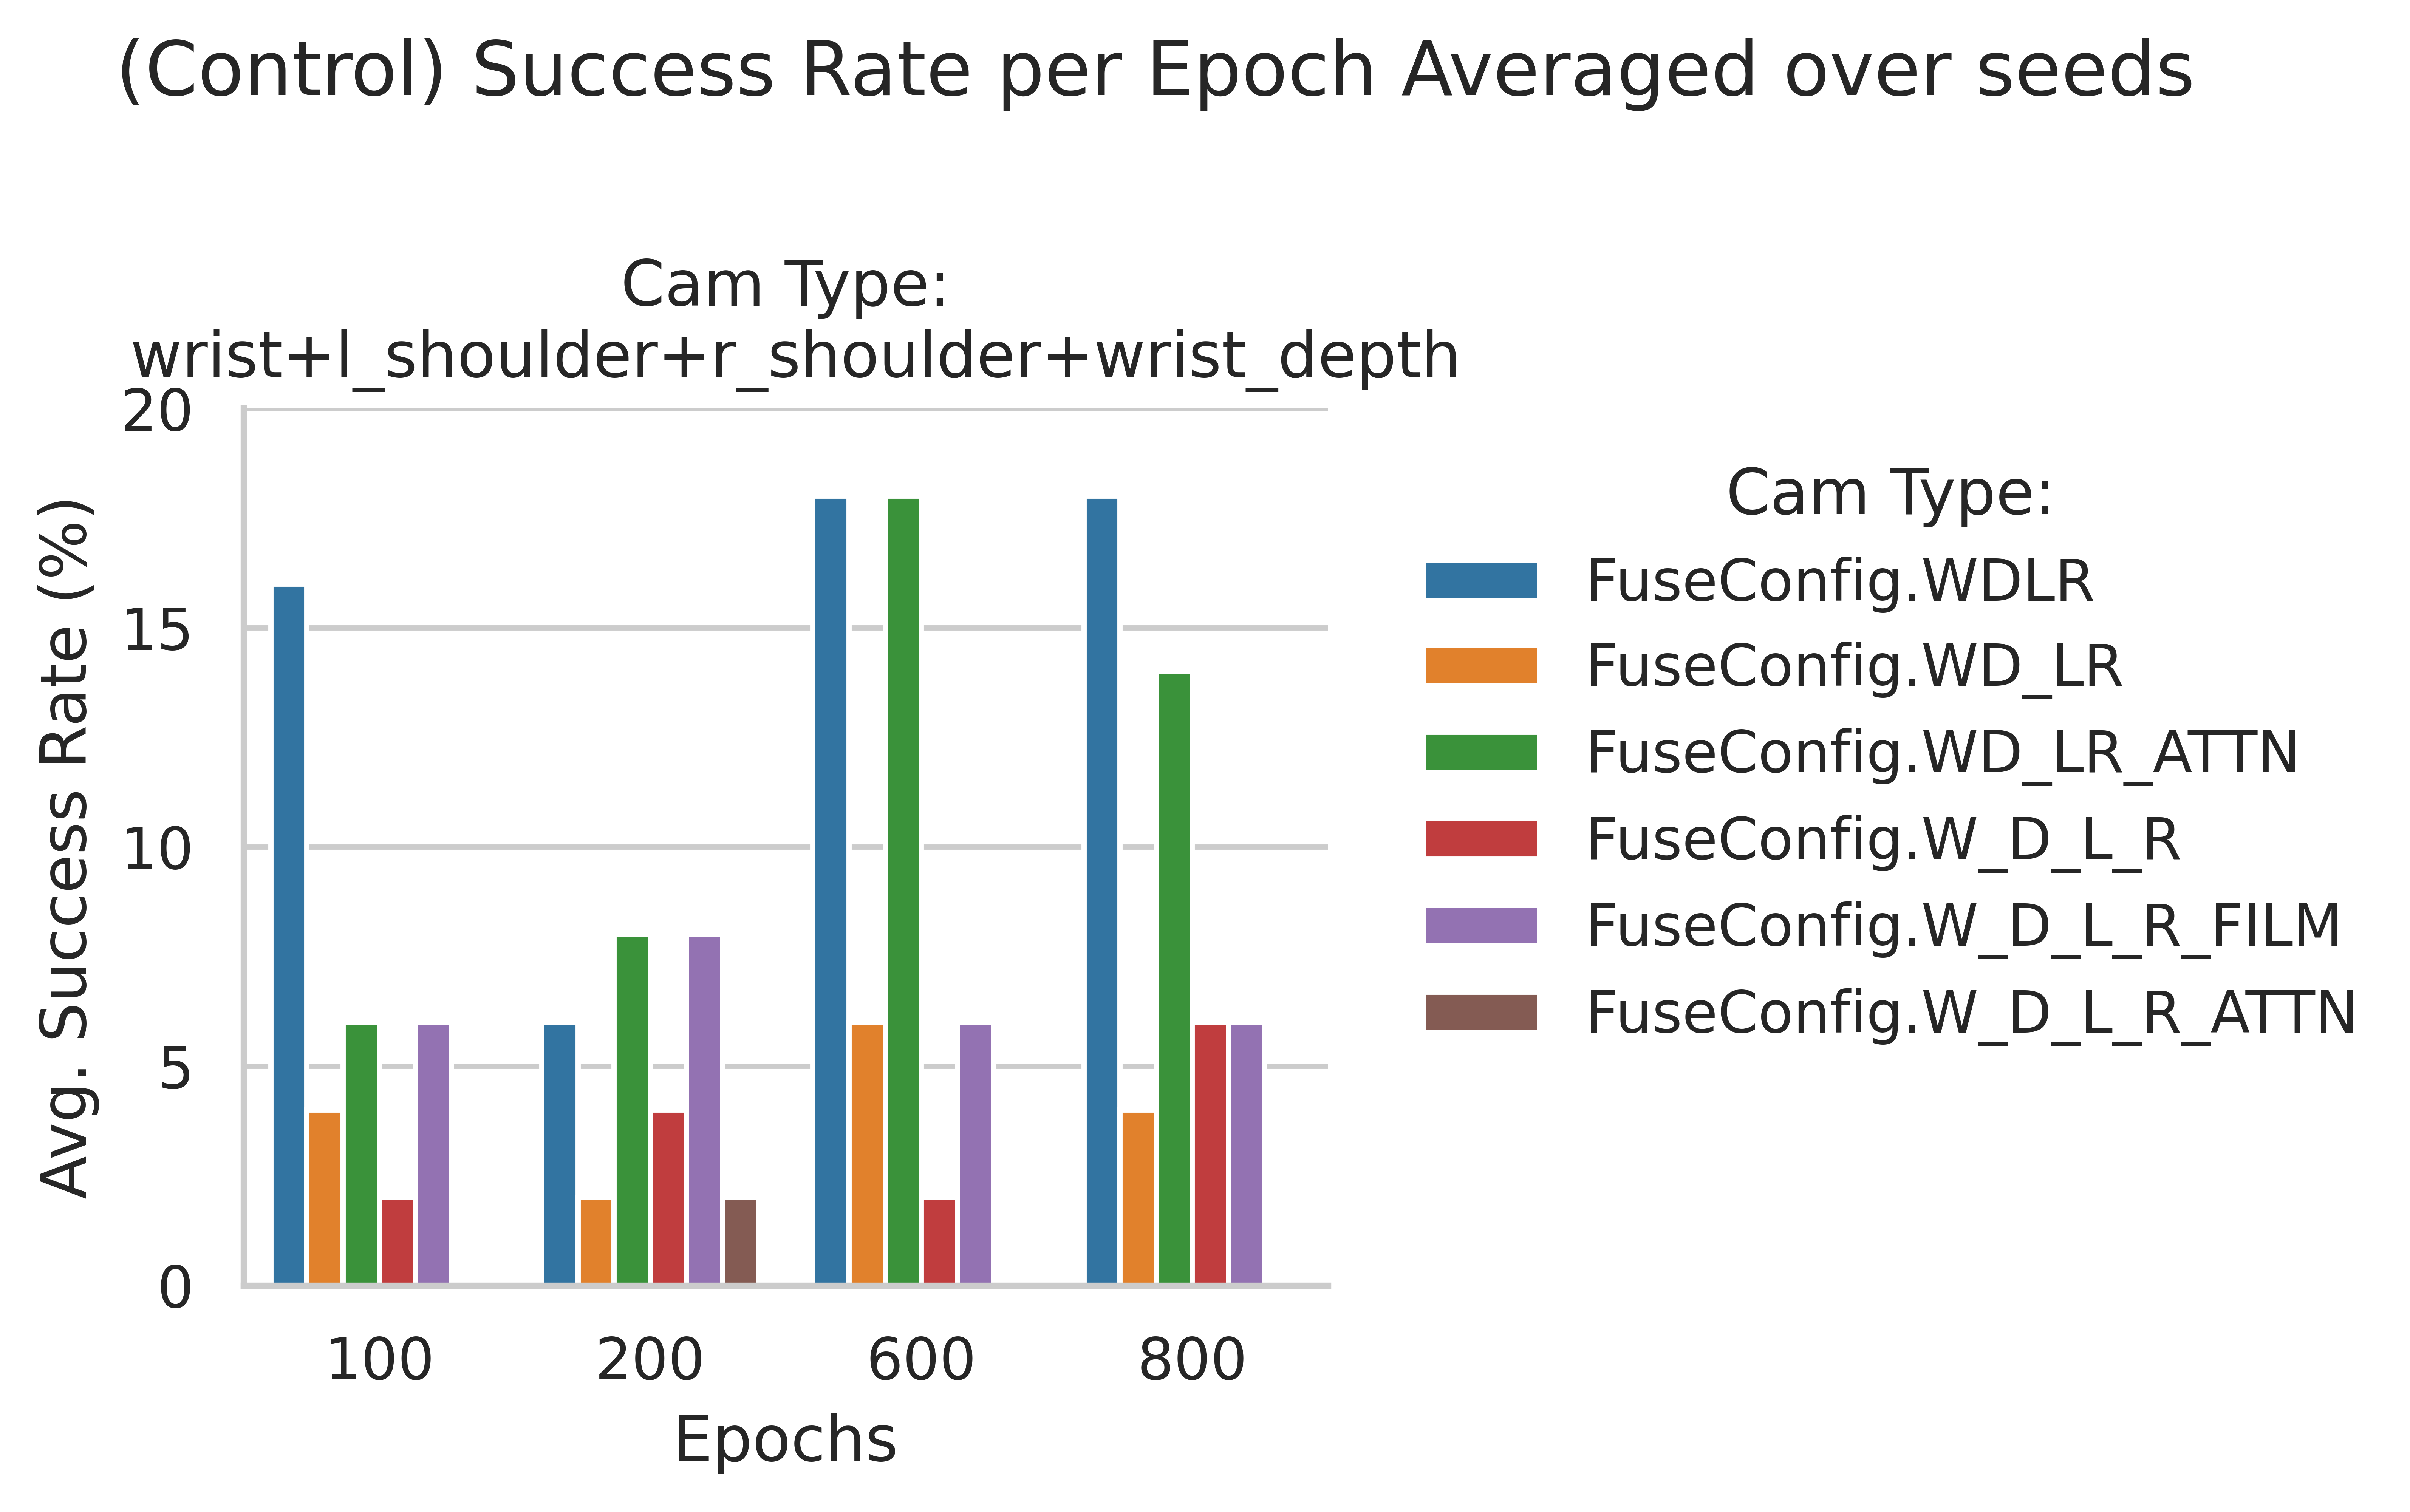
\includegraphics[width=0.4\linewidth]{assets/evaluation/derivatives/grasp-normal-control-success-cams.png}
  \caption{Success rate (\%) for all modalities}\label{fig:derivatives-all-cams-success}
\end{figure}


\begin{figure}[H]
  \centering
  
\includegraphics[width=0.7\linewidth]{assets/evaluation/derivatives/grasp-smaller-final-cams.png}
  \caption{Final Distance Reached for all modalities}\label{fig:deriv-smaller-final-allcams}
\end{figure}

\subsection{Reach with Obstacle}
There wsa nothing of note here, none of the policies here passed the $0.3$ mark consistently while the baseline was averaging around $0.25$. This was also mirrored by the success rate, all the configurations were at most 50\% as successful as baseline, other than \verb|WD_LR| matching it at 100 epochs (with around 43\% overall success). The only significance of this is the highlighted variance in training. As this model does not average a good final distance, but reaches almost half of the tests, this means that the other half, the unsuccessful attempts are going very far from the obstacle, meaning it's failed to generalise to the case of the task.